
%(BEGIN_QUESTION)
% Copyright 2014, Tony R. Kuphaldt, released under the Creative Commons Attribution License (v 1.0)
% This means you may do almost anything with this work of mine, so long as you give me proper credit

A pair of three-phase ``87'' relays -- one at each end of a transmission line -- protects the line from faults along its length.  When initially put into service, the relays immediately trip both circuit breakers to isolate the transmission line, even though subsequent investigations reveal no faults along that line:

$$\includegraphics[width=15.5cm]{i03121x01.eps}$$

Identify the likelihood of each specified fault in this system, to explain why the 87 relays picked up.  Consider each fault one at a time (i.e. no coincidental faults), determining whether or not each fault could independently account for {\it all} observations and symptoms in this circuit.

% No blank lines allowed between lines of an \halign structure!
% I use comments (%) instead, so that TeX doesn't choke.

$$\vbox{\offinterlineskip
\halign{\strut
\vrule \quad\hfil # \ \hfil & 
\vrule \quad\hfil # \ \hfil & 
\vrule \quad\hfil # \ \hfil \vrule \cr
\noalign{\hrule}
%
% First row
{\bf Fault} & {\bf Possible} & {\bf Impossible} \cr
%
\noalign{\hrule}
%
% Another row
Mismatched CT ratios &  &  \cr
%
\noalign{\hrule}
%
% Another row
CT failed open &  &  \cr
%
\noalign{\hrule}
%
% Another row
CT failed shorted &  &  \cr
%
\noalign{\hrule}
%
% Another row
CT wired with wrong polarity &  &  \cr
%
\noalign{\hrule}
%
% Another row
Imbalanced line currents ($I_A \neq I_B \neq I_C$) &  &  \cr
%
\noalign{\hrule}
} % End of \halign 
}$$ % End of \vbox

\underbar{file i03121}
%(END_QUESTION)





%(BEGIN_ANSWER)

% No blank lines allowed between lines of an \halign structure!
% I use comments (%) instead, so that TeX doesn't choke.

$$\vbox{\offinterlineskip
\halign{\strut
\vrule \quad\hfil # \ \hfil & 
\vrule \quad\hfil # \ \hfil & 
\vrule \quad\hfil # \ \hfil \vrule \cr
\noalign{\hrule}
%
% First row
{\bf Fault} & {\bf Possible} & {\bf Impossible} \cr
%
\noalign{\hrule}
%
% Another row
Mismatched CT ratios & $\surd$ &  \cr
%
\noalign{\hrule}
%
% Another row
CT failed open & $\surd$ &  \cr
%
\noalign{\hrule}
%
% Another row
CT failed shorted & $\surd$ &  \cr
%
\noalign{\hrule}
%
% Another row
CT wired with wrong polarity & $\surd$ &  \cr
%
\noalign{\hrule}
%
% Another row
Imbalanced line currents ($I_A \neq I_B \neq I_C$) &  & $\surd$ \cr
%
\noalign{\hrule}
} % End of \halign 
}$$ % End of \vbox

%(END_ANSWER)





%(BEGIN_NOTES)

{\bf This question is intended for exams only and not worksheets!}.

%(END_NOTES)


